\subsection{Cloud Computing}

Cloud computing is a form of distributed computing that turns compute infrastructure, programming
platforms and software systems into scalable utility services. By exposing various compute and programming
resources as utility services, cloud computing promotes resource sharing at scale via the Internet.
Depending on the type of resources
offered as services, cloud computing platforms can be categorized into three main categories:

\begin{description}
\item [Infrastructure-as-a-Service clouds (IaaS)]
Offers low-level compute, storage and networking
resources as a service. Compute resources are typically provided in the form of on-demand virtual machines 
with specific CPU, memory and disk configurations (e.g. Amazon EC2, Google Compute Engine, Eucalyptus). 
\item [Platform-as-a-Service clouds (PaaS)]
Offers a programming platform as a service, that can be used to develop and deploy applications at scale 
(e.g. Google App Engine, AppScale, Heroku, Amazon Elastic Beanstalk).
\item [Software-as-a-Service clouds (SaaS)]
Offers a collection of software applications and tools as a service, that can be directly consumed by
application endusers (e.g. Salesforce, Workday, Citrix go2meeting). This can be thought of as a new way 
of delivering software to
endusers. Instead of prompting the users to download and install any software, SaaS enables the users
to consume software via the Internet.  
\end{description}

Due to the benefits associated with cloud computing (scalability, high availability, productivity enhancement etc.),
many developers and organizations have adopted the cloud as their preferred means of developing, deploying and
delivering software applications. Such cloud-hosted applications expose one or more web application programming 
interfaces (web APIs) through which users can remotely interact with the applications. A cloud-hosted 
application may
also consume web APIs exposed by other cloud-hosted applications. Thus, cloud-hosted applications
form an intricate graph of inter-dependencies among them, where each application can service a set of
applications, while being dependent on a set of other applications. However, in general, each cloud-hosted
application directly depends on the core services offered by the underlying cloud platform for compute power, storage,
network connectivity and scalability.

In the next subsection we take a closer look at a specific type of cloud platforms -- Platform-as-a-Service clouds.
We use PaaS clouds as a case study and a testbed in a number of our explorations.

\subsection{Platform-as-a-Service Clouds}
PaaS clouds provide a managed application programming platform, where an application developer can simply 
write some code, and run it at scale at the push of a button. It relieves the developer from having to install or configure
any hardware resources, virtual machines or operating systems. Moreover, PaaS clouds do not require the developers
to set up any utility services their applications might require such as a database or a distributed cache. 
Everything an application requires is provisioned and managed by the PaaS cloud.

\begin{figure}
\centering
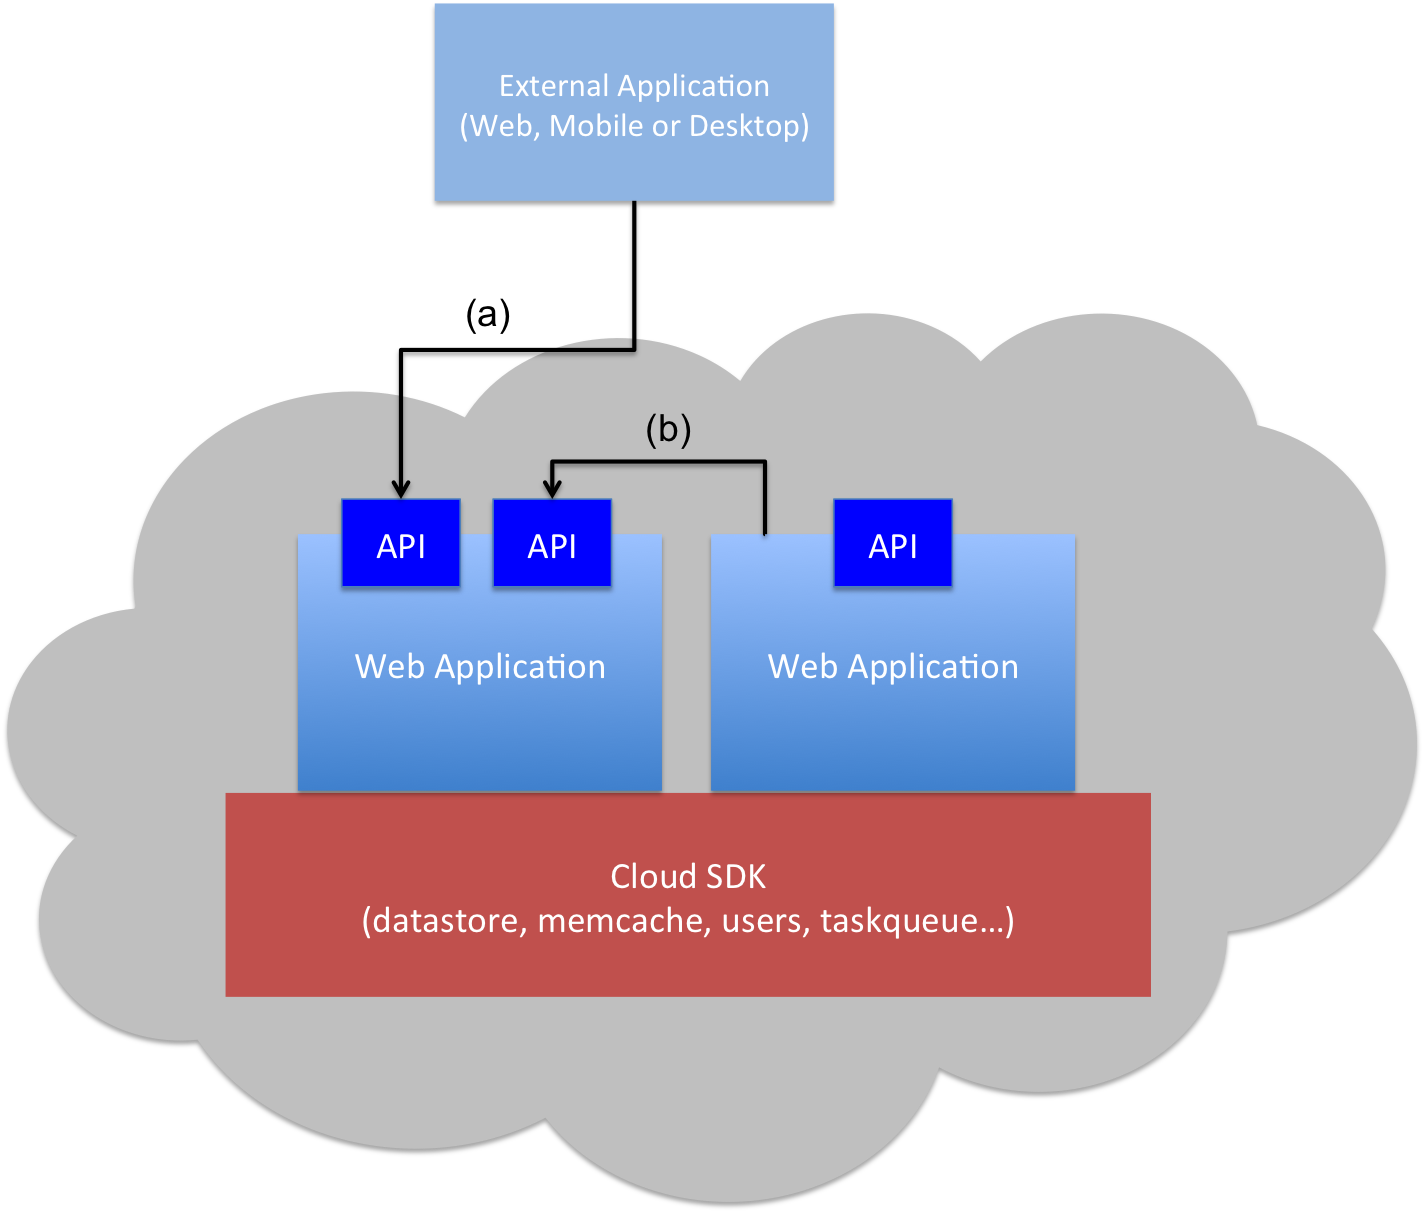
\includegraphics[scale=0.35]{cloud_app_model}
\caption{Applications deployed in a PaaS cloud: (a) An external client making requests
to an application via the web API;
(b) A PaaS-hosted application invoking another in the same cloud.
\label{fig:cloud_app_model}
}
\vspace{-0.2in}
\end{figure}

Figure~\ref{fig:cloud_app_model} provides a graphical overview of a PaaS cloud. 
The cloud platform provides a base 
framework, called cloud SDK (software development kit), on which new applications can be developed. 
The cloud SDK 
is a set of high level programming APIs, with abstractions for common application services such as data storage, caching, 
user management and more. The developer uses these abstractions to implement his/her application logic, and packages 
it as a web application. The service implementations for the 
cloud SDK are highly scalable, highly available (have SLAs associated with them),
and automatically managed by the platform. Developers then
upload their applications to the cloud for deployment.
Once deployed, the applications and any web APIs exported by them can be accessed 
via HTTP/S requests by external or co-located clients.

PaaS clouds are specifically built for deploying and running applications -- 
applications that are directly consumed by end users and other client applications. This means, all the problems 
outlined in the previous section, such as poor development practices, performance SLAs and performance 
debugging directly impact PaaS clouds. Therefore PaaS clouds are ideal candidates for implementing the type
of governance systems proposed in this work. 

We use PaaS clouds in our research extensively both as case studies
and experimental platforms. Specifically, we use Google App Engine and AppScale as test environments
to experiment with our new governance systems. App Engine is a highly scalable public PaaS cloud hosted and
managed by Google in their data centers. While it is open for anyone to deploy and run web applications, it is not
open source software, and its internal deployment details are not commonly known. AppScale is open source
software that can be used to set up a private cloud platform on one's own physical or virtual hardware. AppScale
is API compatible with App Engine (i.e. it supports the same cloud SDK), and hence any web application developed
for App Engine can be deployed on AppScale without any code changes. In our experiments, we typically deploy
AppScale over a small cluster of physical machines, or over a set of virtual machines provided by an IaaS cloud
such as Eucalyptus.

By experimenting with real world PaaS clouds we demonstrate the practical feasibility and the effectiveness of 
the systems we design and implement. Furthermore, there are currently over a million applications deployed
in App Engine, with a significant proportion of them being open source applications. Therefore we have access
to a large number of real world PaaS applications to experiment with.

\subsection{Governance}
\subsubsection{IT and SOA Governance}
Traditionally, information and technology (IT) governance~\cite{brown2005framing} has been a branch of 
corporate governance, focused on
improving performance and managing the risks associated with the use of information and technology. The primary
goals of IT governance are three fold:

\begin{itemize}
\item Assure that the use of IT generates business value
\item Oversee performance of IT usage and management
\item Mitigate the risks of using IT
\end{itemize}

A number of frameworks, models and even certification systems have emerged over time to help organizations 
implement IT governance. When the software engineering community started gravitating towards web services and
service-oriented computing (SOC)~\cite{1254461, what-is-soa}, a new type of digital assets rose to prominence within corporate IT 
infrastructures -- ``services''. Aggregates of loosely-coupled, reusable, modular services soon replaced 
large monolithic software
installations. Services required new forms of governance for managing their performance
and risks. Hence the notion of service-oriented architecture (SOA) governance came into existence. 

Multiple definitions of SOA governance
are in circulation, but most of them agree that the purpose of SOA governance is to exercise control over
services and associated processes (service development, testing, monitoring etc). A commonly used definition
of SOA governance is ensuring and validating that service artifacts within the architecture are operating
as expected and maintaining a certain level of quality~\cite{gartner-soa-gov}.
Consequently, a number of tools that help organizations implement SOA governance 
have also evolved.
Since web services are the mostly widely used form of services in SOA-driven systems, most of these
SOA governance tools have a strong focus on controlling web services. 

Policies play a crucial role in all forms of governance. A policy is a specification of the acceptable behavior
of some entity. The entity could be a department, a software system, a service or a 
human process such as developing
a new application. In SOA governance, policies state how services should be developed, how they are to be
deployed, how to secure them and what level of quality-of-service to maintain while a service is in operation.
SOA governance tools enable administrators to specify acceptable service behavior and life-cycle as policies, and
a software policy enforcement agent automatically enacts those policies to control various aspects of the 
services. 

\subsubsection{Governance for Cloud-hosted Applications}
Cloud computing can be thought of as a heightened version of service-oriented computing. While classic
SOC strives to offer data and application functionality as services, cloud computing offers a variety
of additional computing resources
as services including hardware infrastructure (compute power, storage space and networking) and programming
platforms. Moreover, the applications deployed on cloud platforms are typically implemented as services with
separate implementation and interface components. The web APIs exposed by these applications play the
role of the service interface.
Much like classic services, each cloud-hosted application 
can be a dependency for another
co-located cloud application, or an application running elsewhere (e.g. a mobile agent). 
Due to this resemblance, many concepts related to SOA governance are
directly applicable to cloud platforms and cloud-hosted applications. For instance, we can envision an 
automated policy enforcement agent enacting a 
set of policies that control the behavior and the life-cycle of cloud-hosted applications.

More specifically, we are interested in using policies to control the following aspects of cloud-hosted 
applications.
\begin{enumerate}
\item Development and deployment conventions (including dependency management, naming and packaging
standards and backward compatibility)
\item Performance SLAs offered to the users
\item Diagnosing performance bugs and bottlenecks
\end{enumerate}

Our research focuses on using automated policy enforcement, diagnostics and other related 
governance features to ensure that
cloud-hosted applications adhere to developer best practices and administrative conventions, while
consistently meeting performance expectations of the developers and the users. We strive to design
governance mechanisms that scale up well to handle cloud workloads -- i.e. large numbers of applications
and policies. We build on existing SOC and cloud computing research, and introduce novel methods
where existing governance and detection methods fall short. 